In this section the central shapes of the two analysis grounps( Alpha and A ) are compared.  
Data templates have raw yields. All background templates are normalized to a unit area so that one can 
compare shapes, not normalization. All templates are for \mHi=125 \GeV analysis.

\begin{figure}[!hbtp]
\centering

\subfigure[Data]{
\centering
\label{subfig:data_0j}
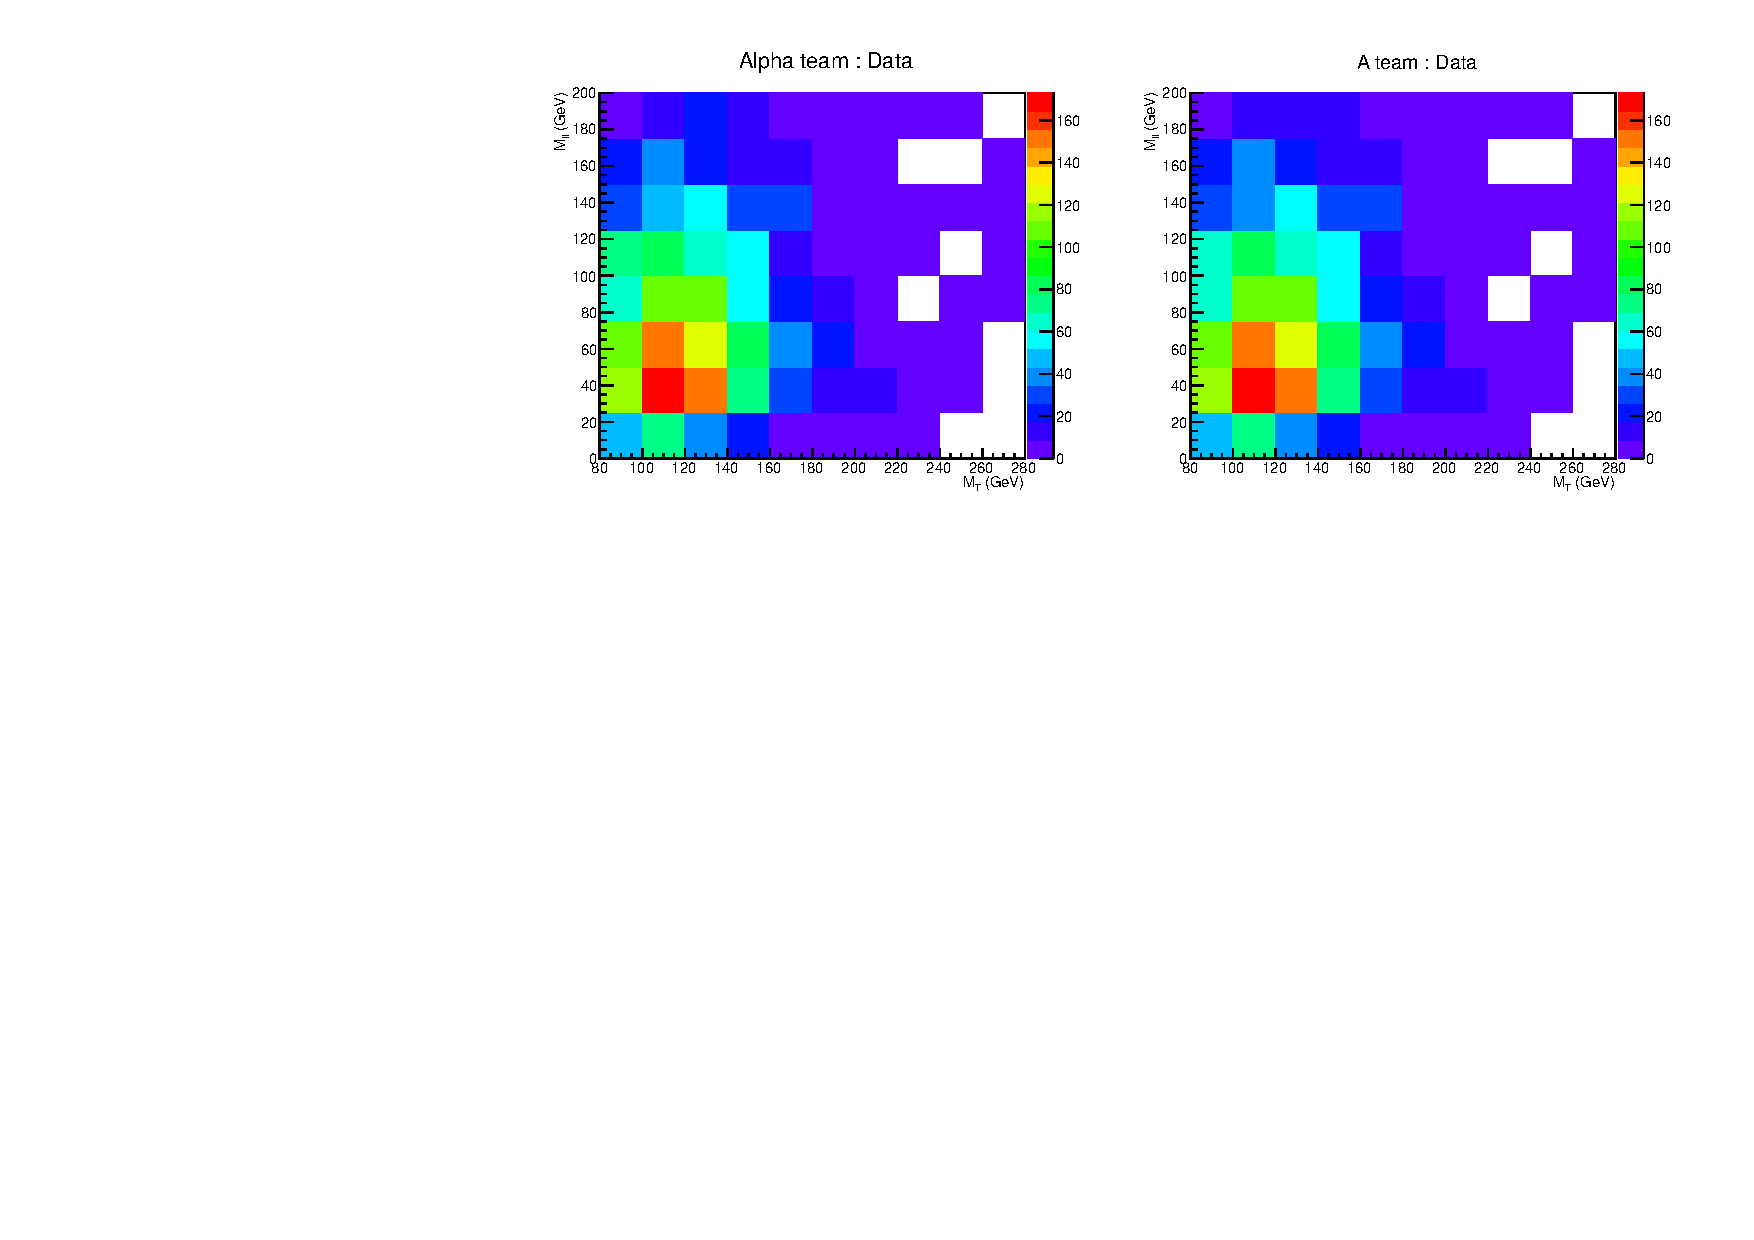
\includegraphics[width=.8\textwidth]{figures/compare_Data_0j.pdf}
} \\
\subfigure[qqWW]{
\centering
\label{subfig:qqWW_0j}
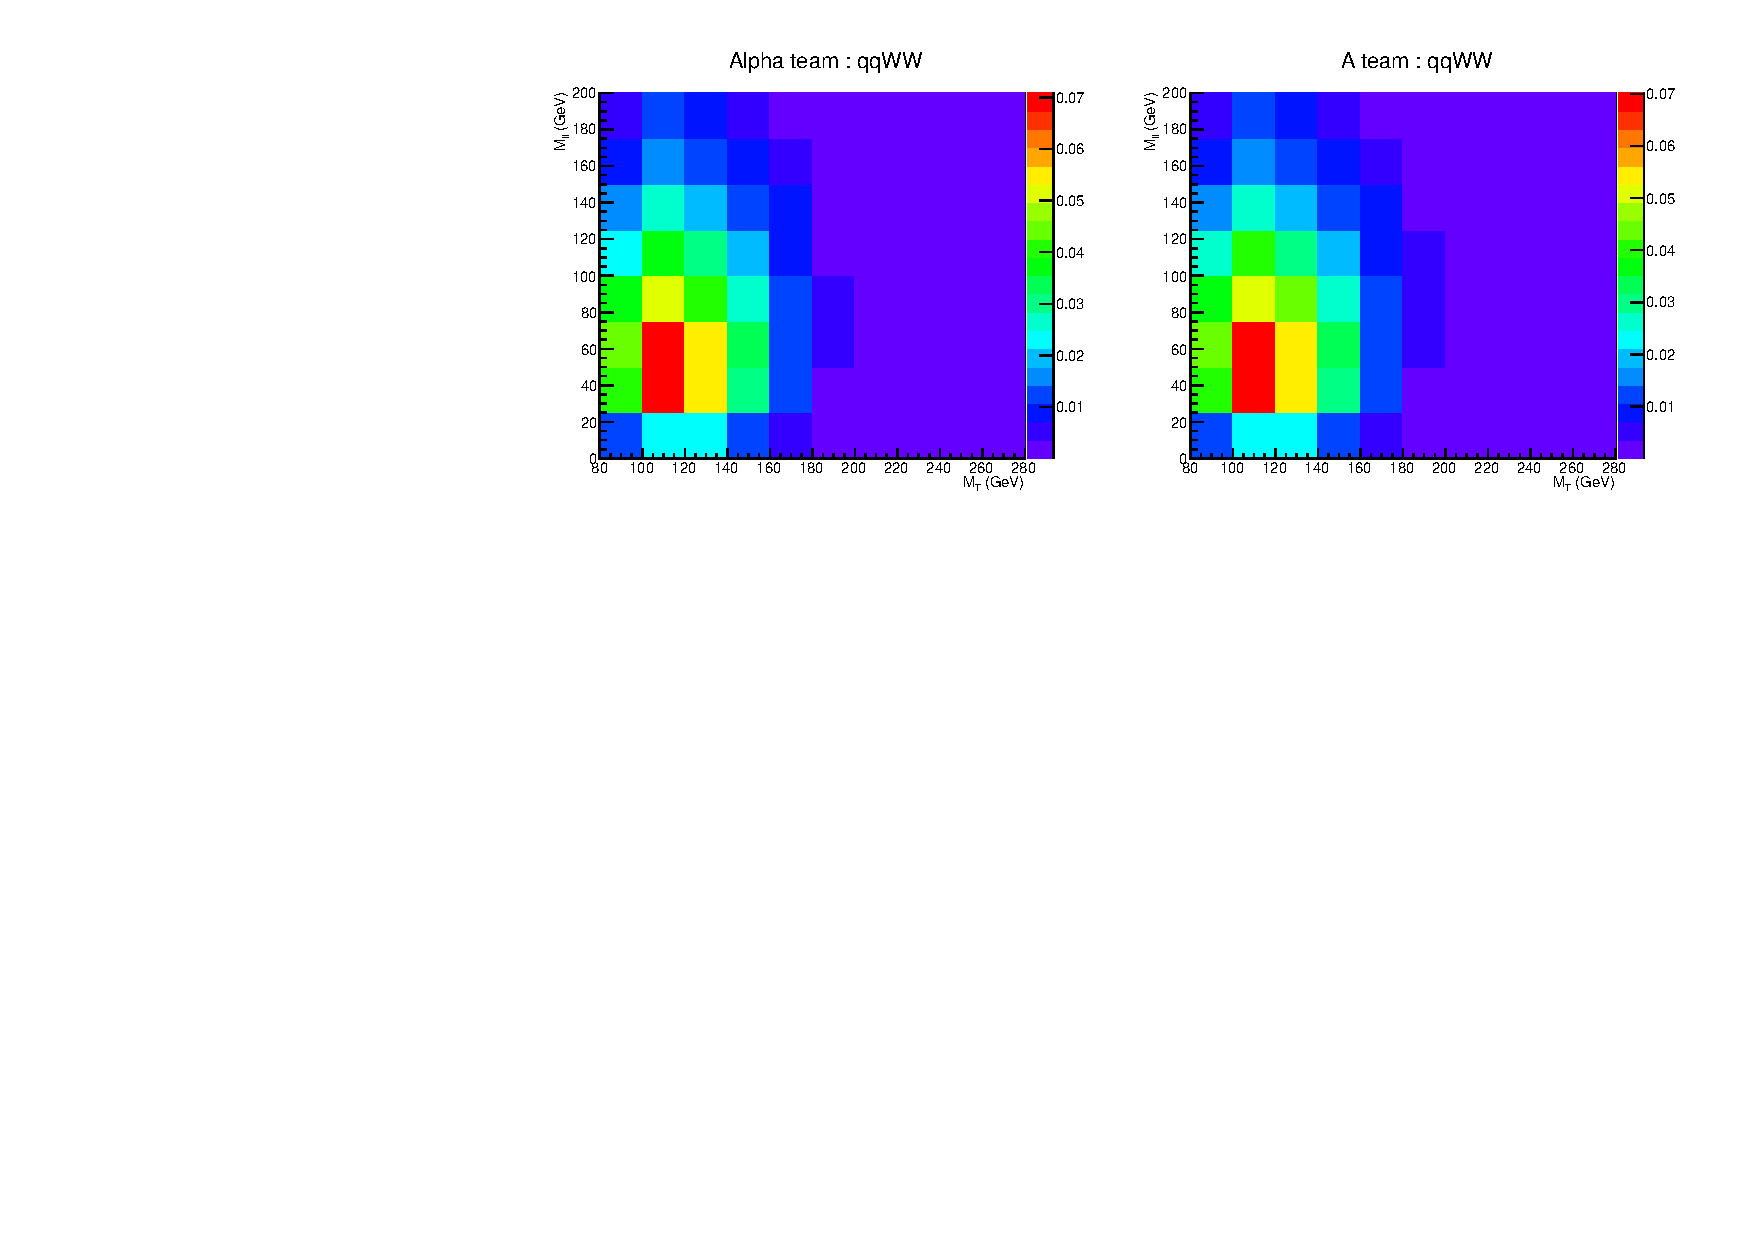
\includegraphics[width=.8\textwidth]{figures/compare_qqWW_0j.pdf}
} \\
\subfigure[ggWW]{
\centering
\label{subfig:ggWW_0j}
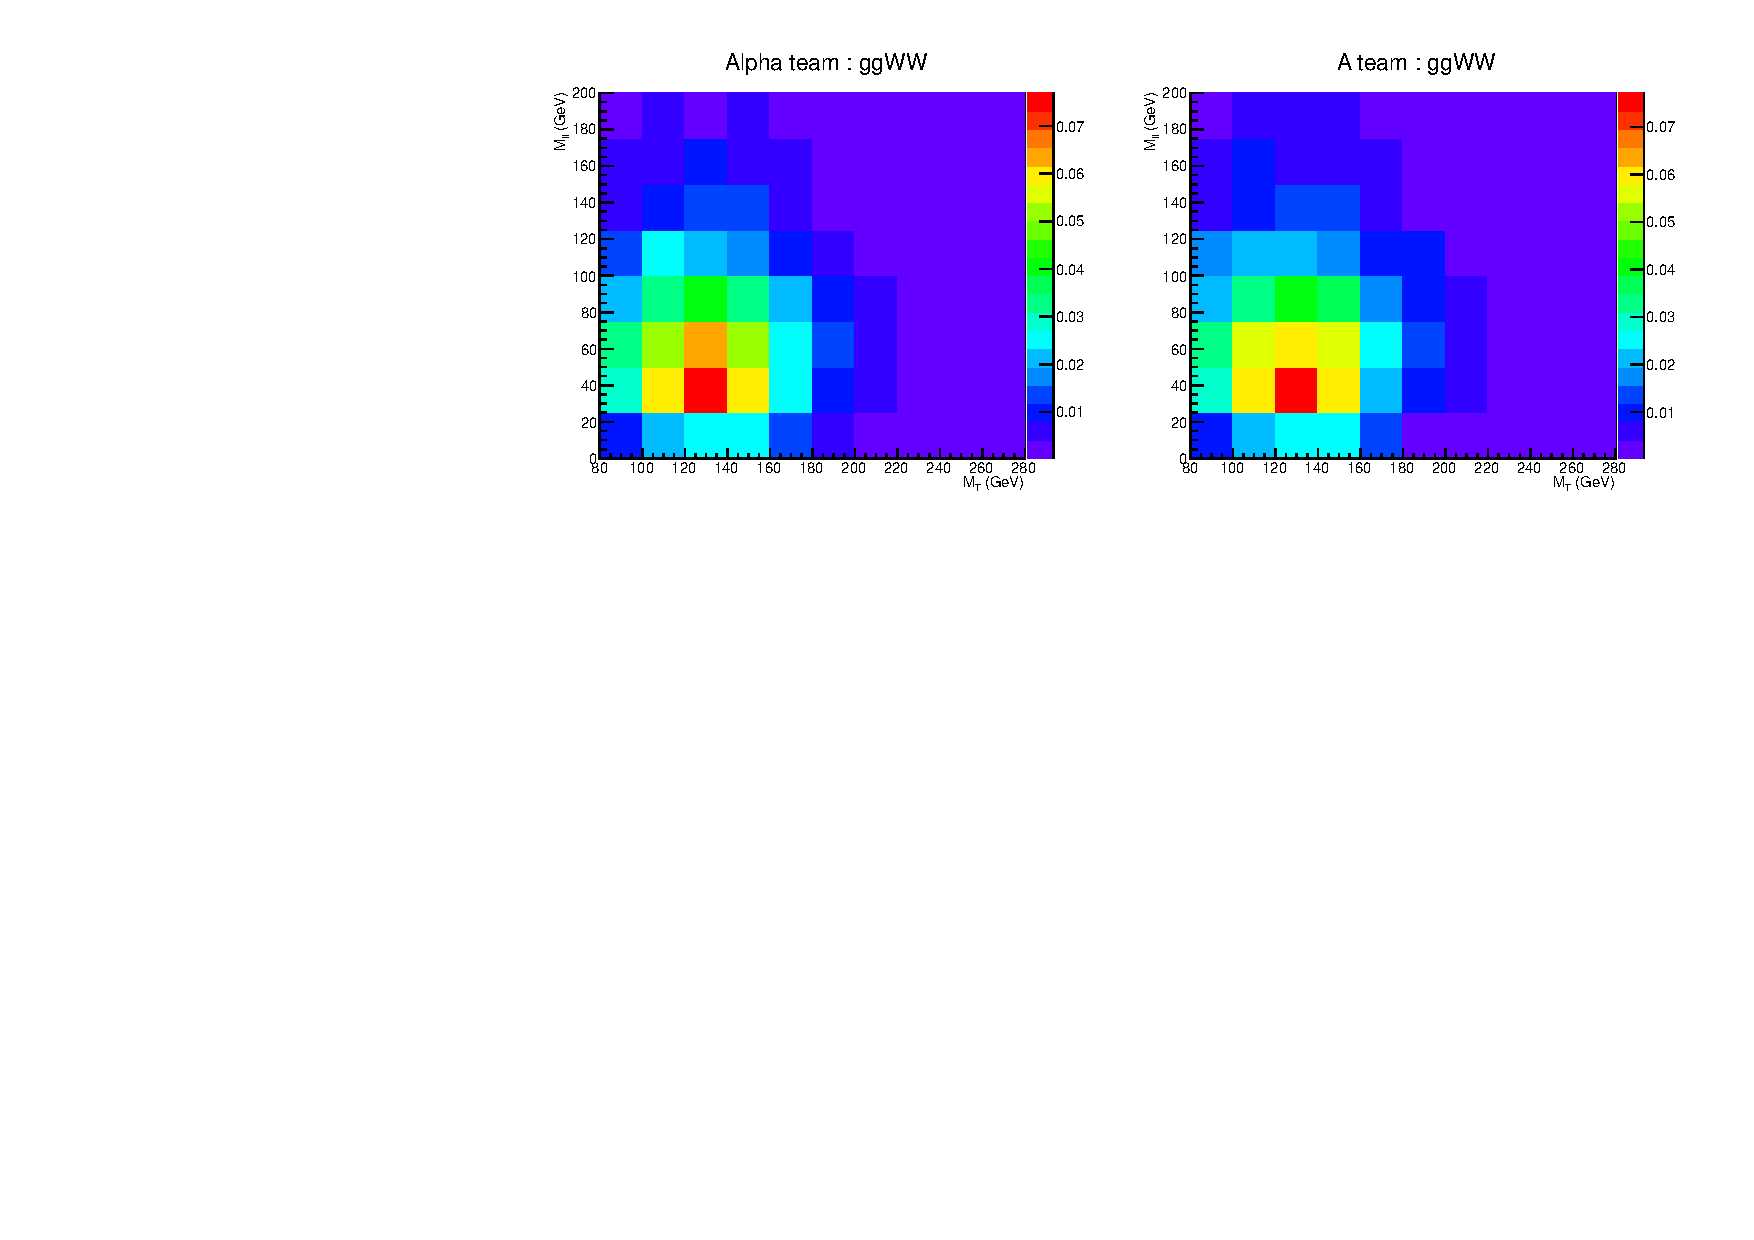
\includegraphics[width=.8\textwidth]{figures/compare_ggWW_0j.pdf}
} \\

\caption{ The 2D ($m_{ll}, m_T$) templates for the Alpha team and A team in the 0-Jet bin with $m_H<300$ GeV. }
\label{fig:compare_temlates_0j}
\end{figure}

\begin{figure}[!hbtp]
\centering

\subfigure[Top]{
\centering
\label{subfig:Top_0j}
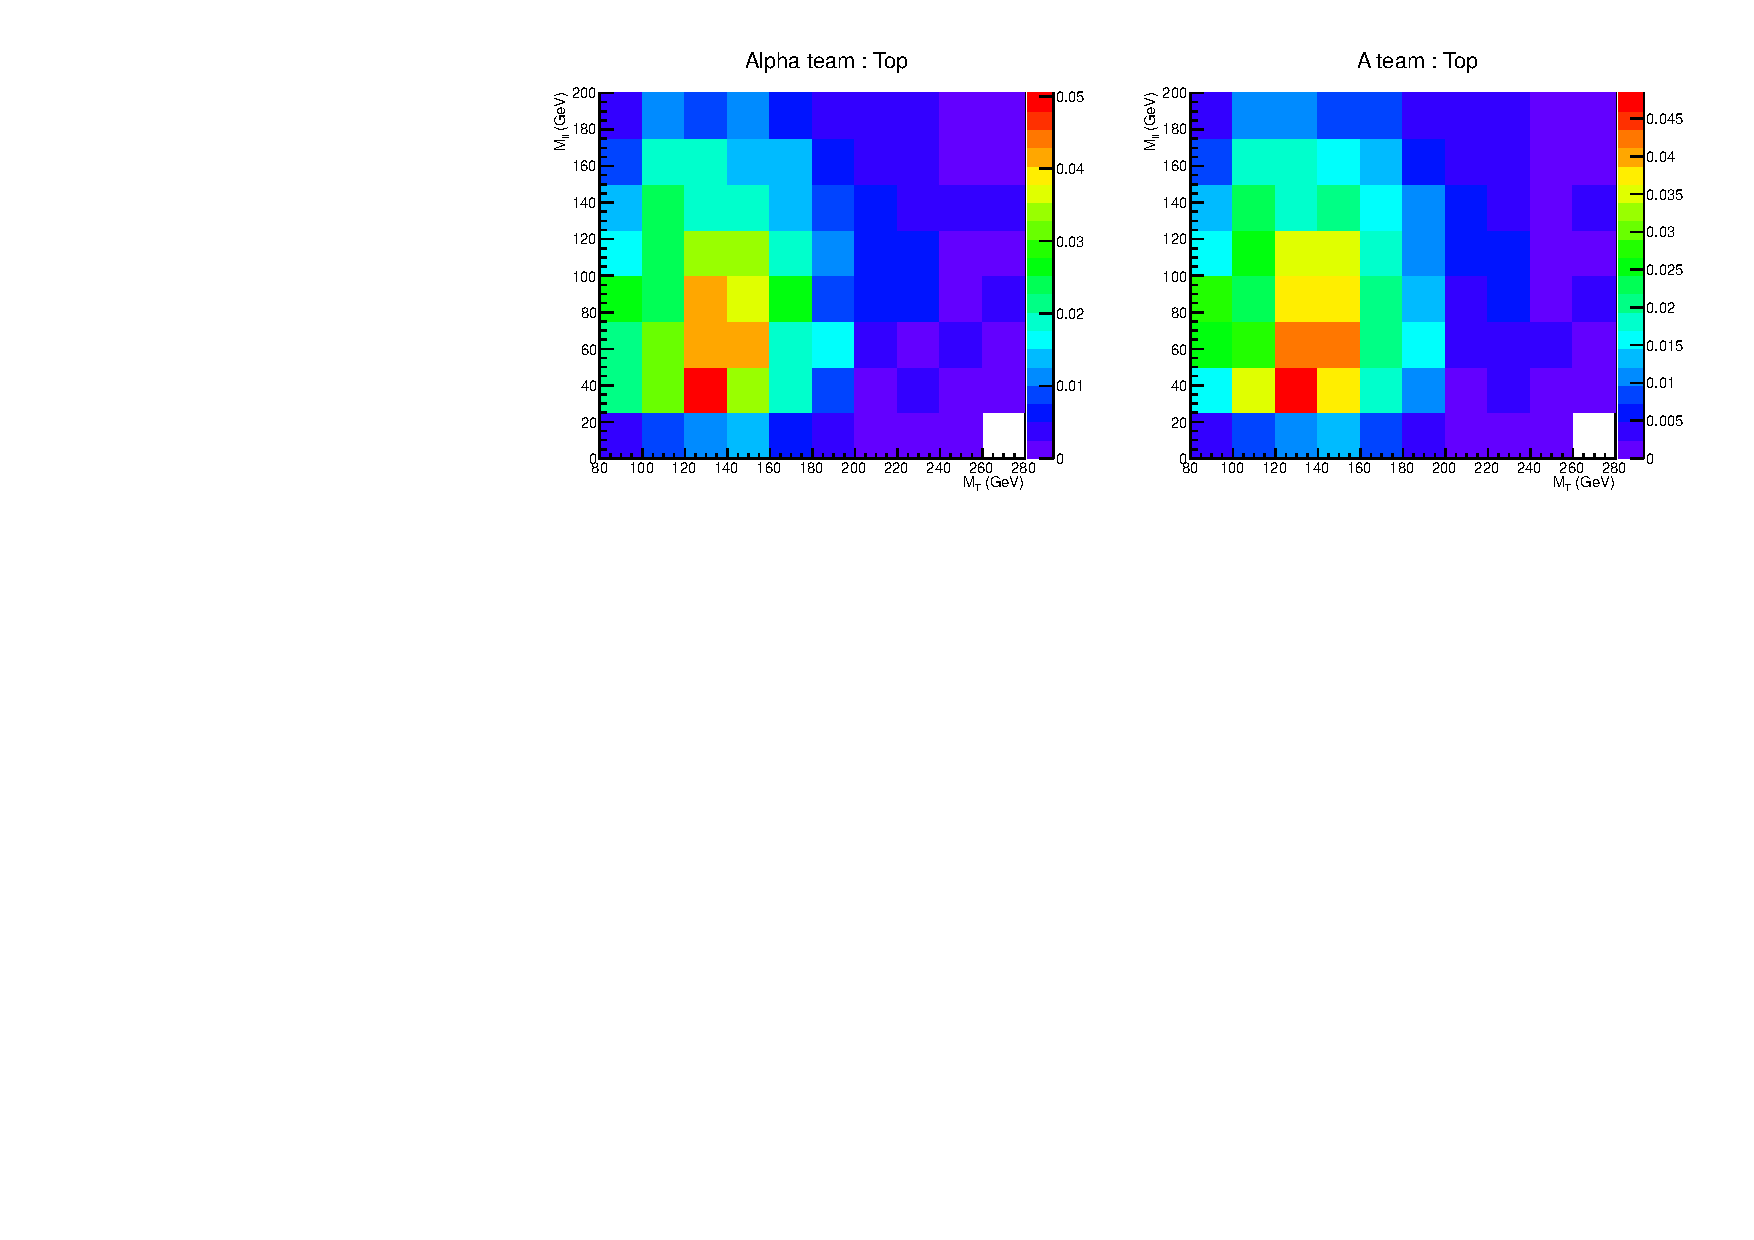
\includegraphics[width=.8\textwidth]{figures/compare_Top_0j.pdf}
} \\
\subfigure[Wjets]{
\centering
\label{subfig:Wjets_0j}
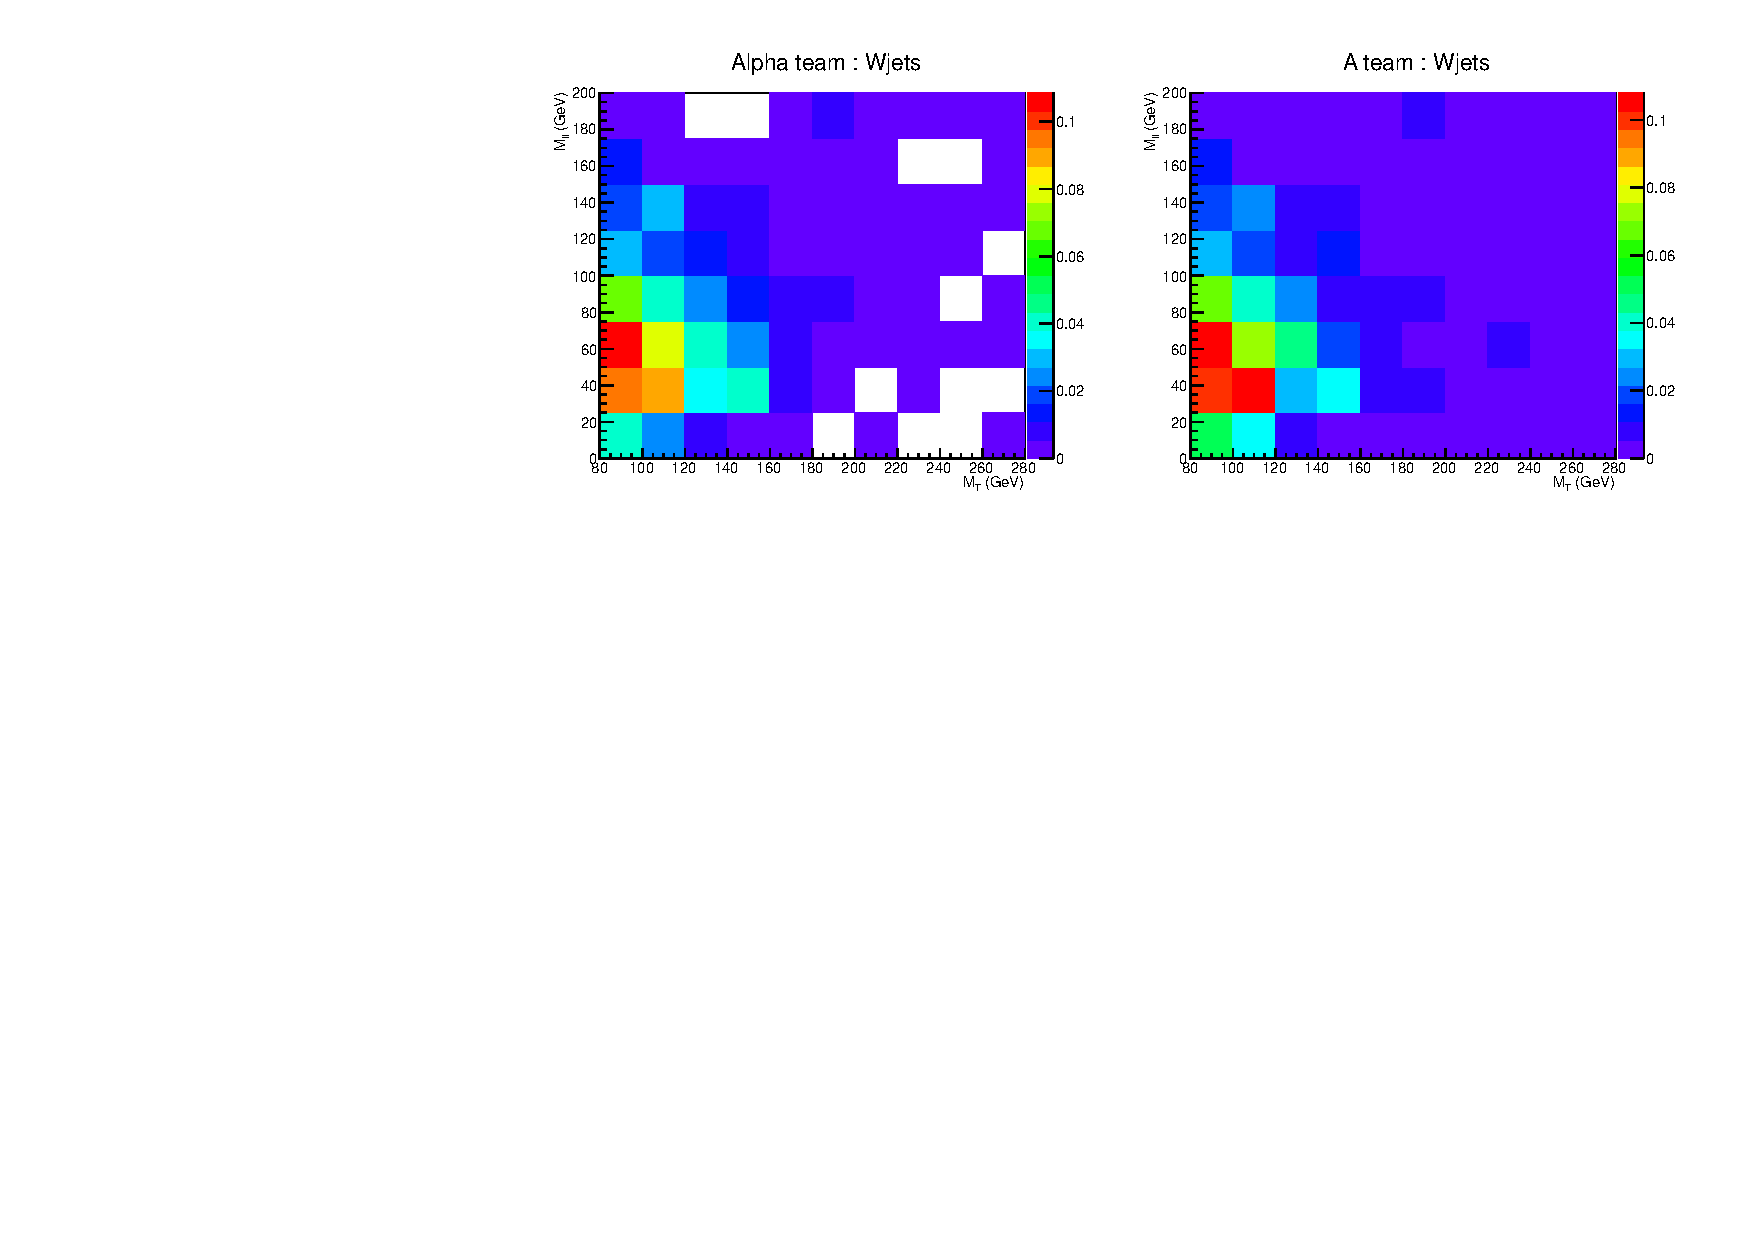
\includegraphics[width=.8\textwidth]{figures/compare_Wjets_0j.pdf}
} \\
\subfigure[Wgamma]{
\centering
\label{subfig:Wgamma_0j}
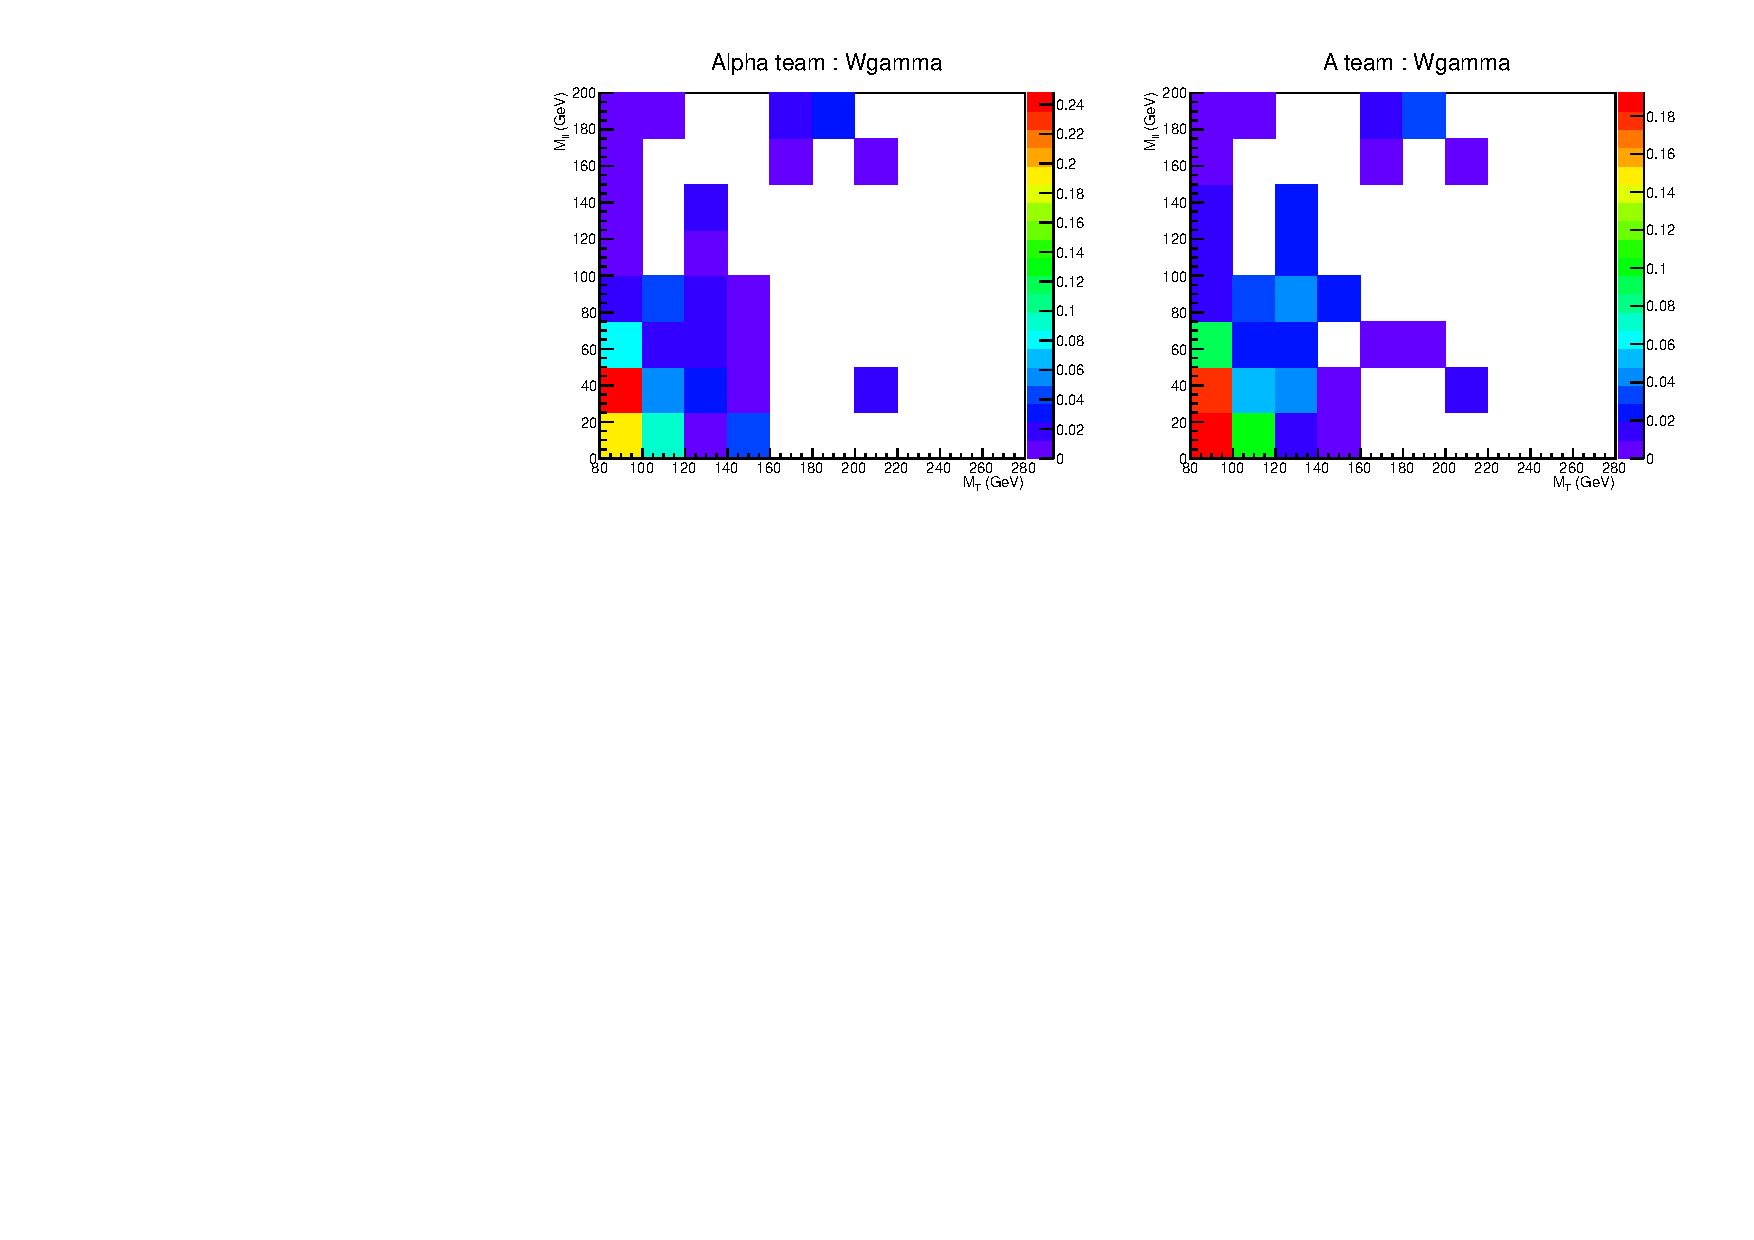
\includegraphics[width=.8\textwidth]{figures/compare_Wgamma_0j.pdf}
} \\

\caption{ The 2D ($m_{ll}, m_T$) templates for the Alpha team and A team in the 0-Jet bin with $m_H<300$ GeV. }
\label{fig:compare_temlates_0j}
\end{figure}

%%%%%
\begin{figure}[!hbtp]
\centering

\subfigure[Data]{
\centering
\label{subfig:data_1j}
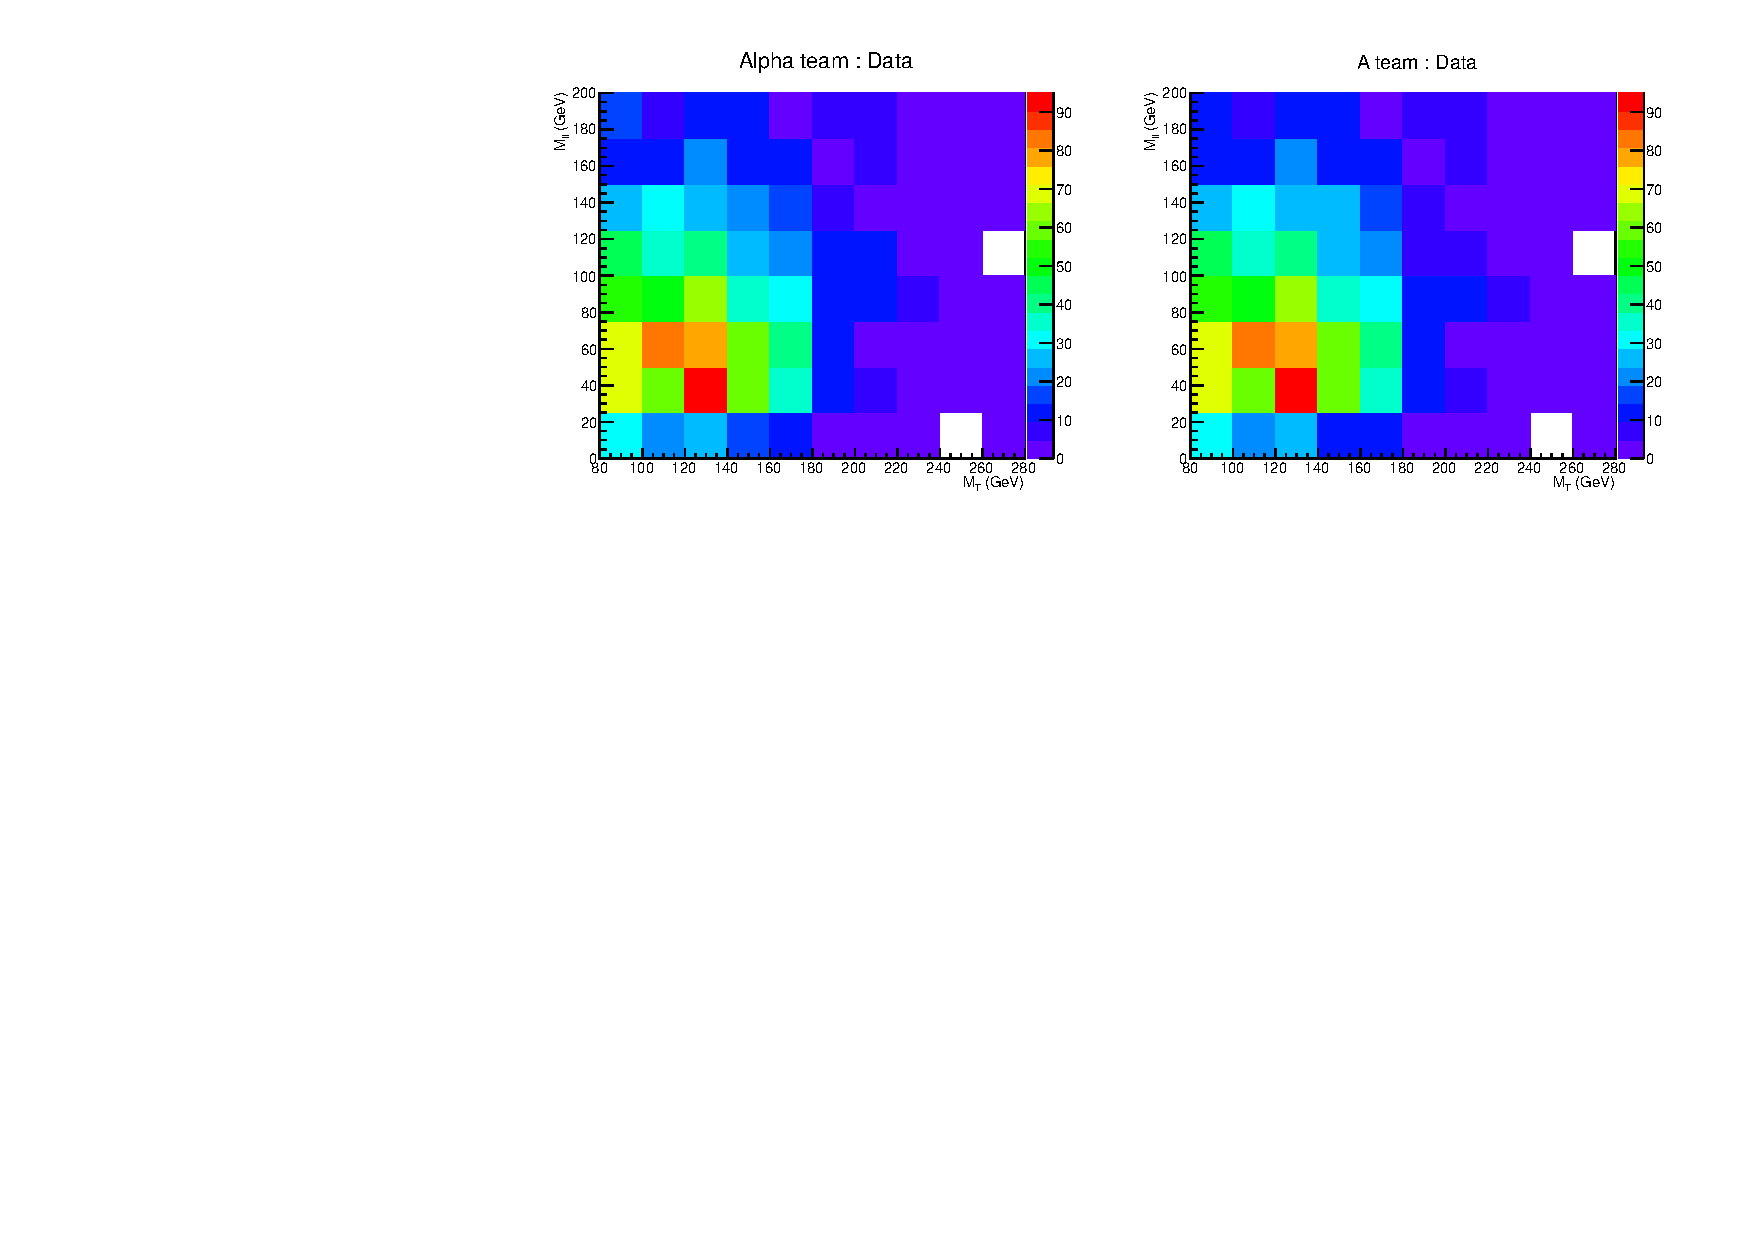
\includegraphics[width=.8\textwidth]{figures/compare_Data_1j.pdf}
} \\
\subfigure[qqWW]{
\centering
\label{subfig:qqWW_1j}
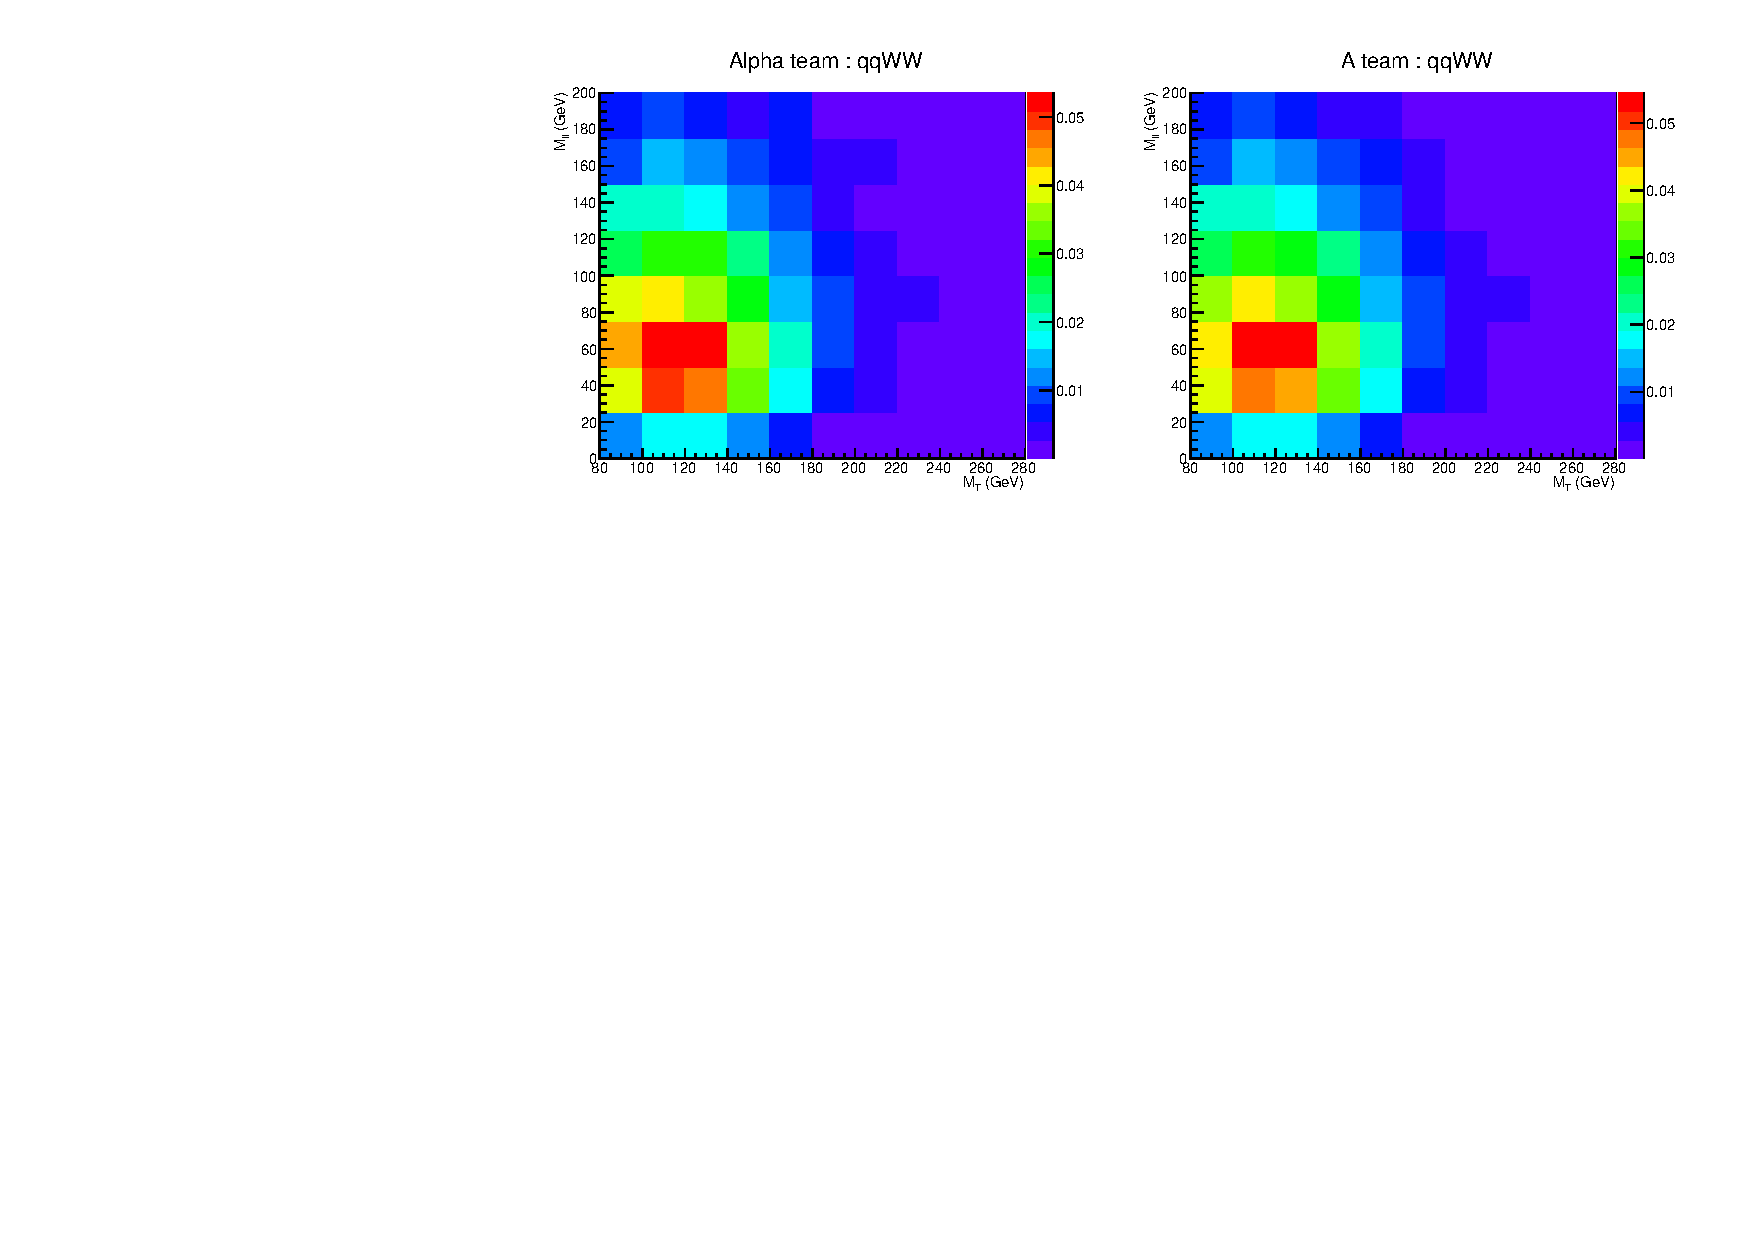
\includegraphics[width=.8\textwidth]{figures/compare_qqWW_1j.pdf}
} \\
\subfigure[ggWW]{
\centering
\label{subfig:ggWW_1j}
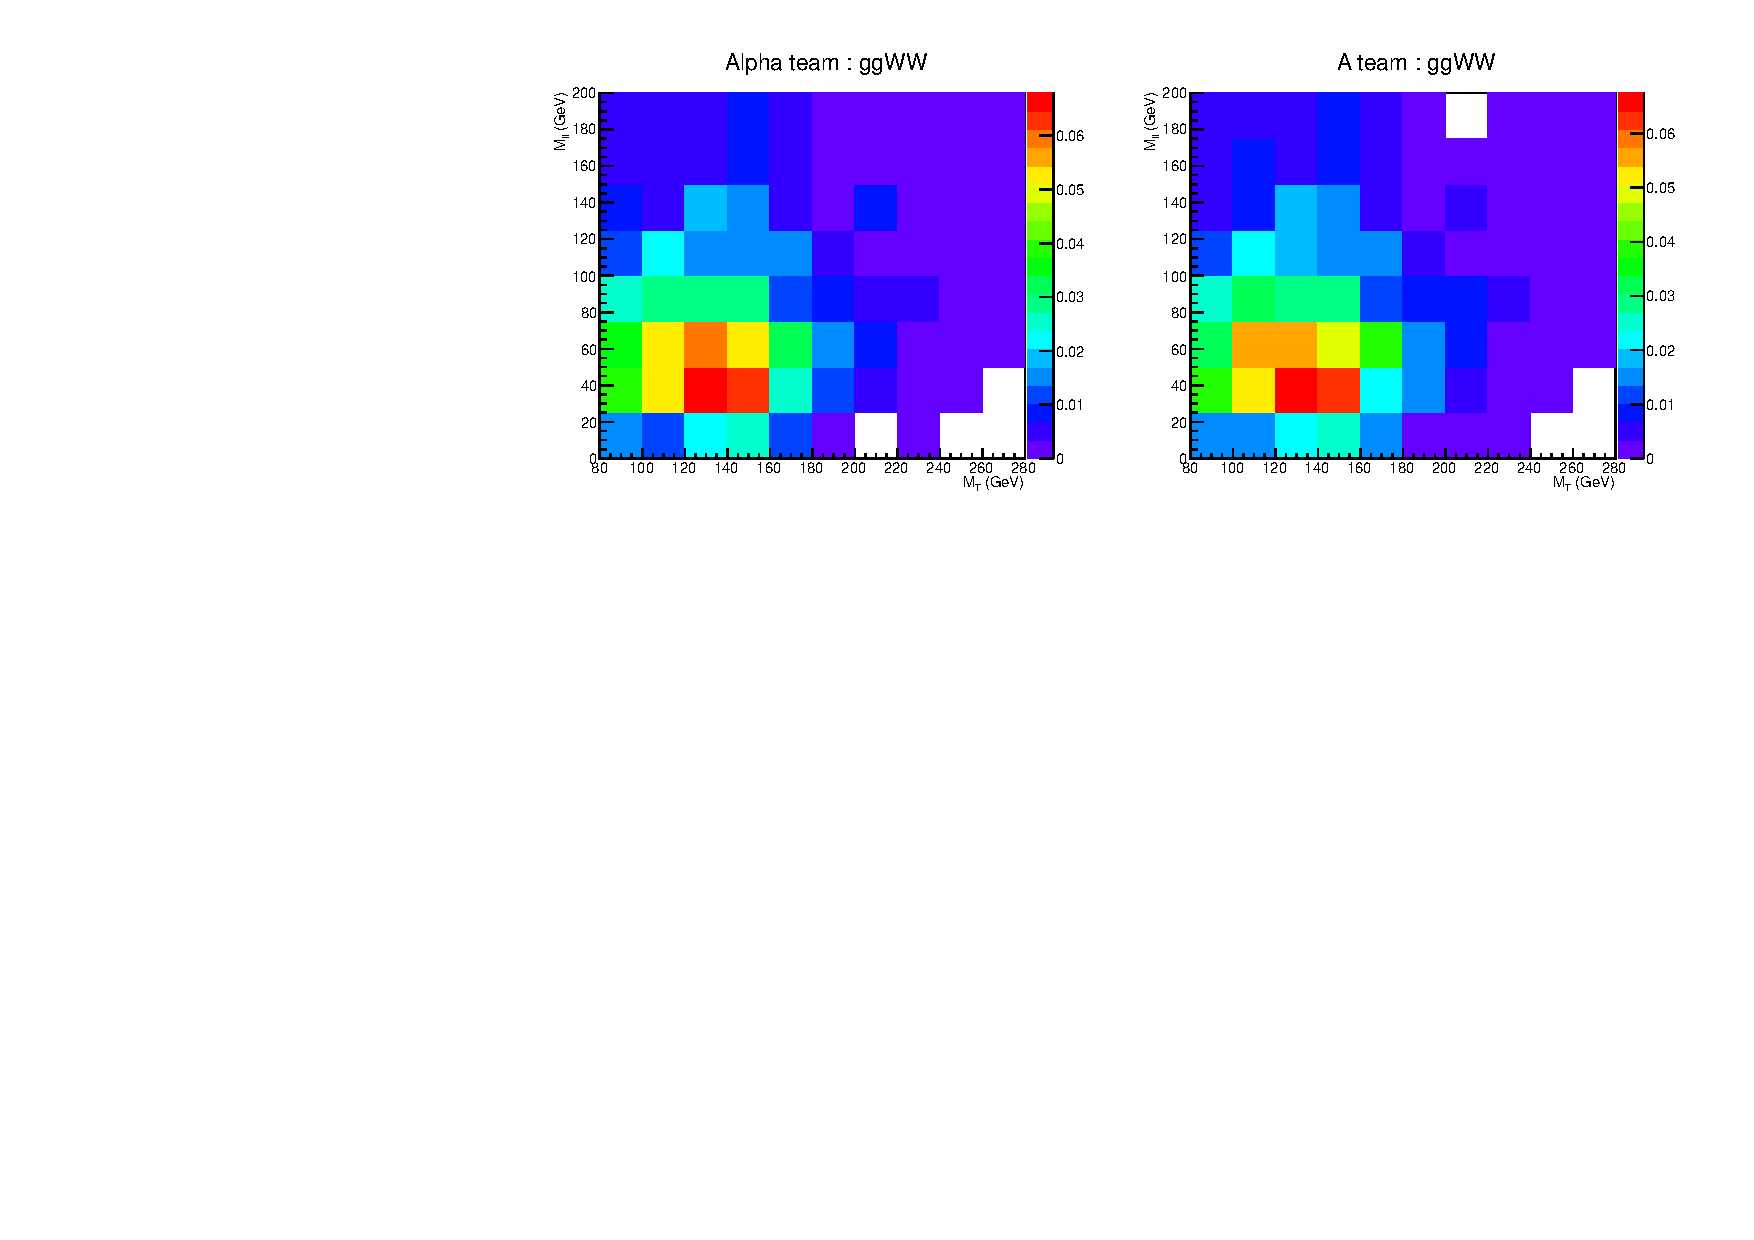
\includegraphics[width=.8\textwidth]{figures/compare_ggWW_1j.pdf}
} \\

\caption{ The 2D ($m_{ll}, m_T$) templates for the Alpha team and A team in the 0-Jet bin with $m_H<300$ GeV. }
\label{fig:compare_temlates_0j}
\end{figure}

\begin{figure}[!hbtp]
\centering
\subfigure[Top]{
\centering
\label{subfig:Top_1j}
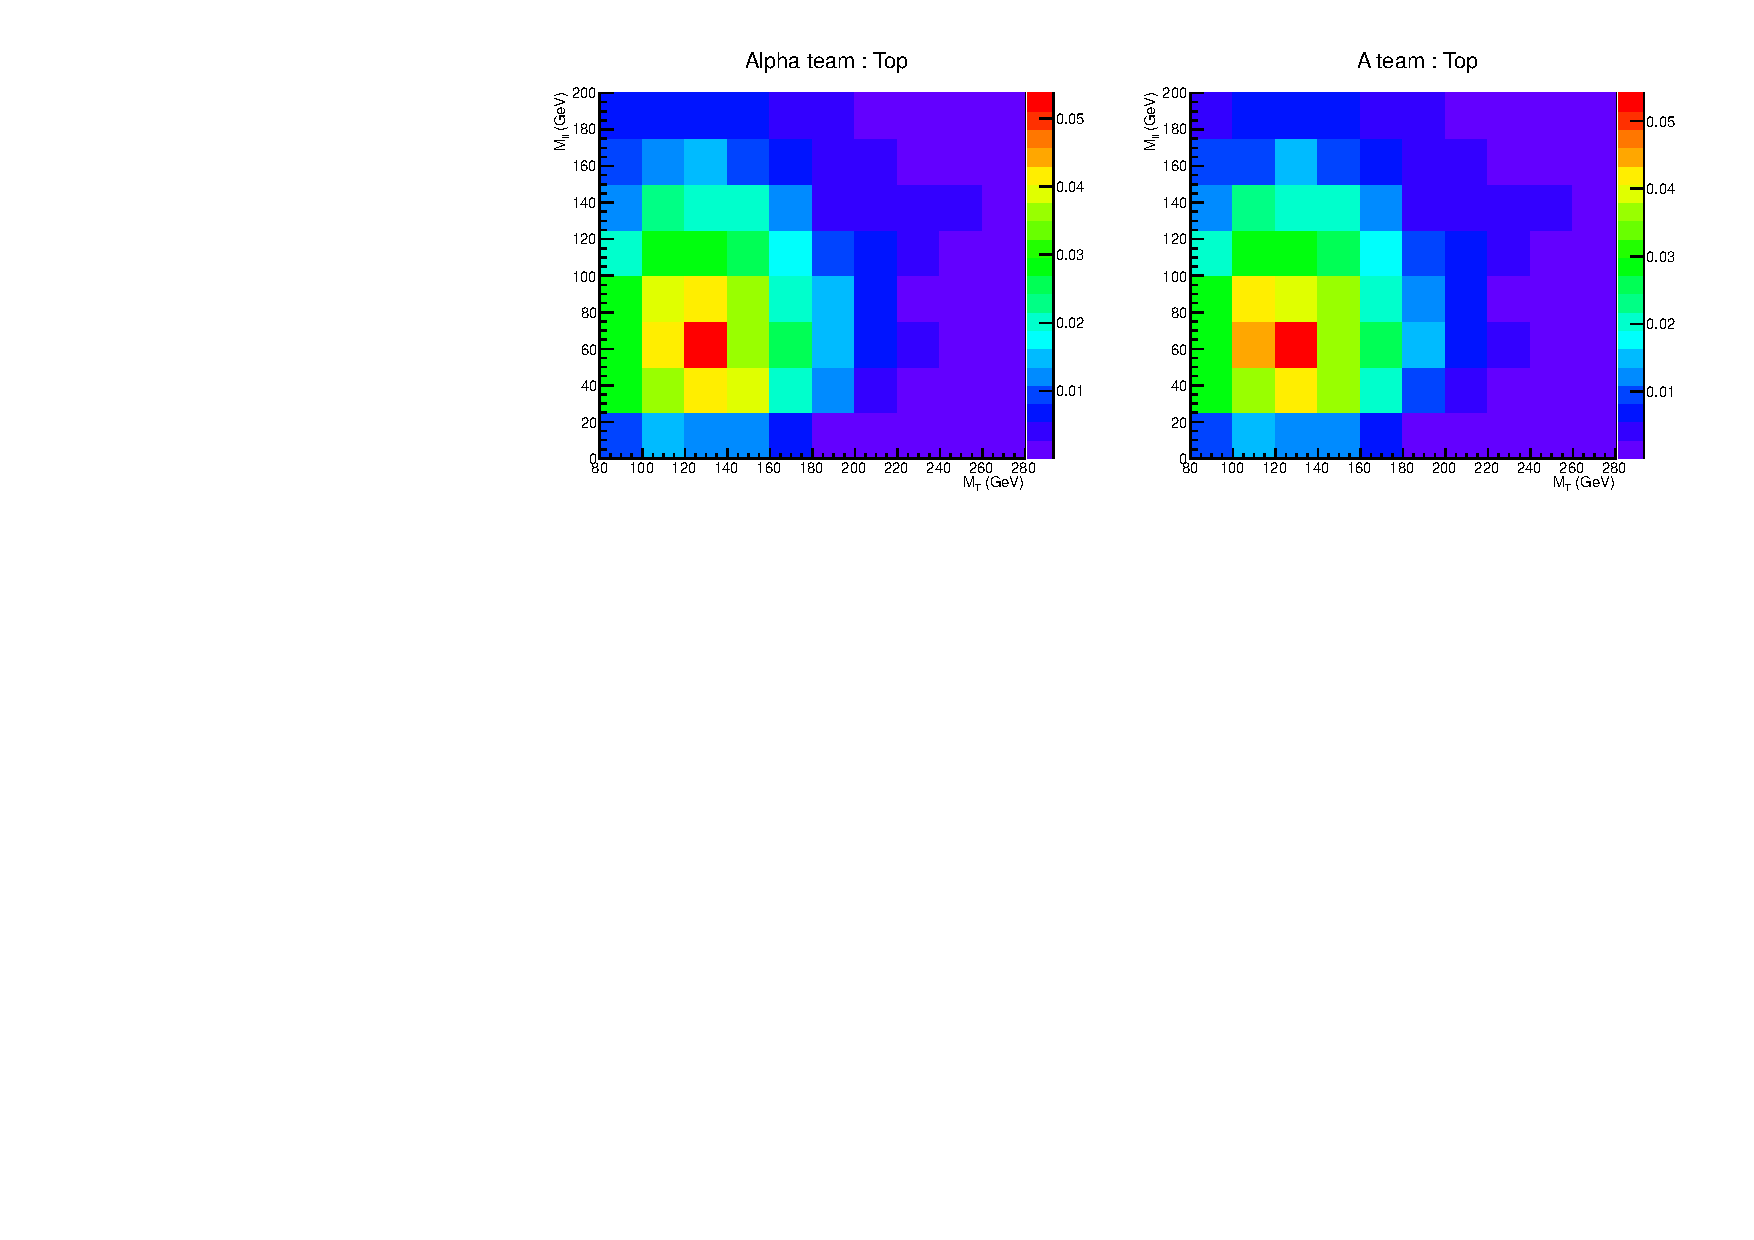
\includegraphics[width=.8\textwidth]{figures/compare_Top_1j.pdf}
} \\
\subfigure[Wjets]{
\centering
\label{subfig:Wjets_1j}
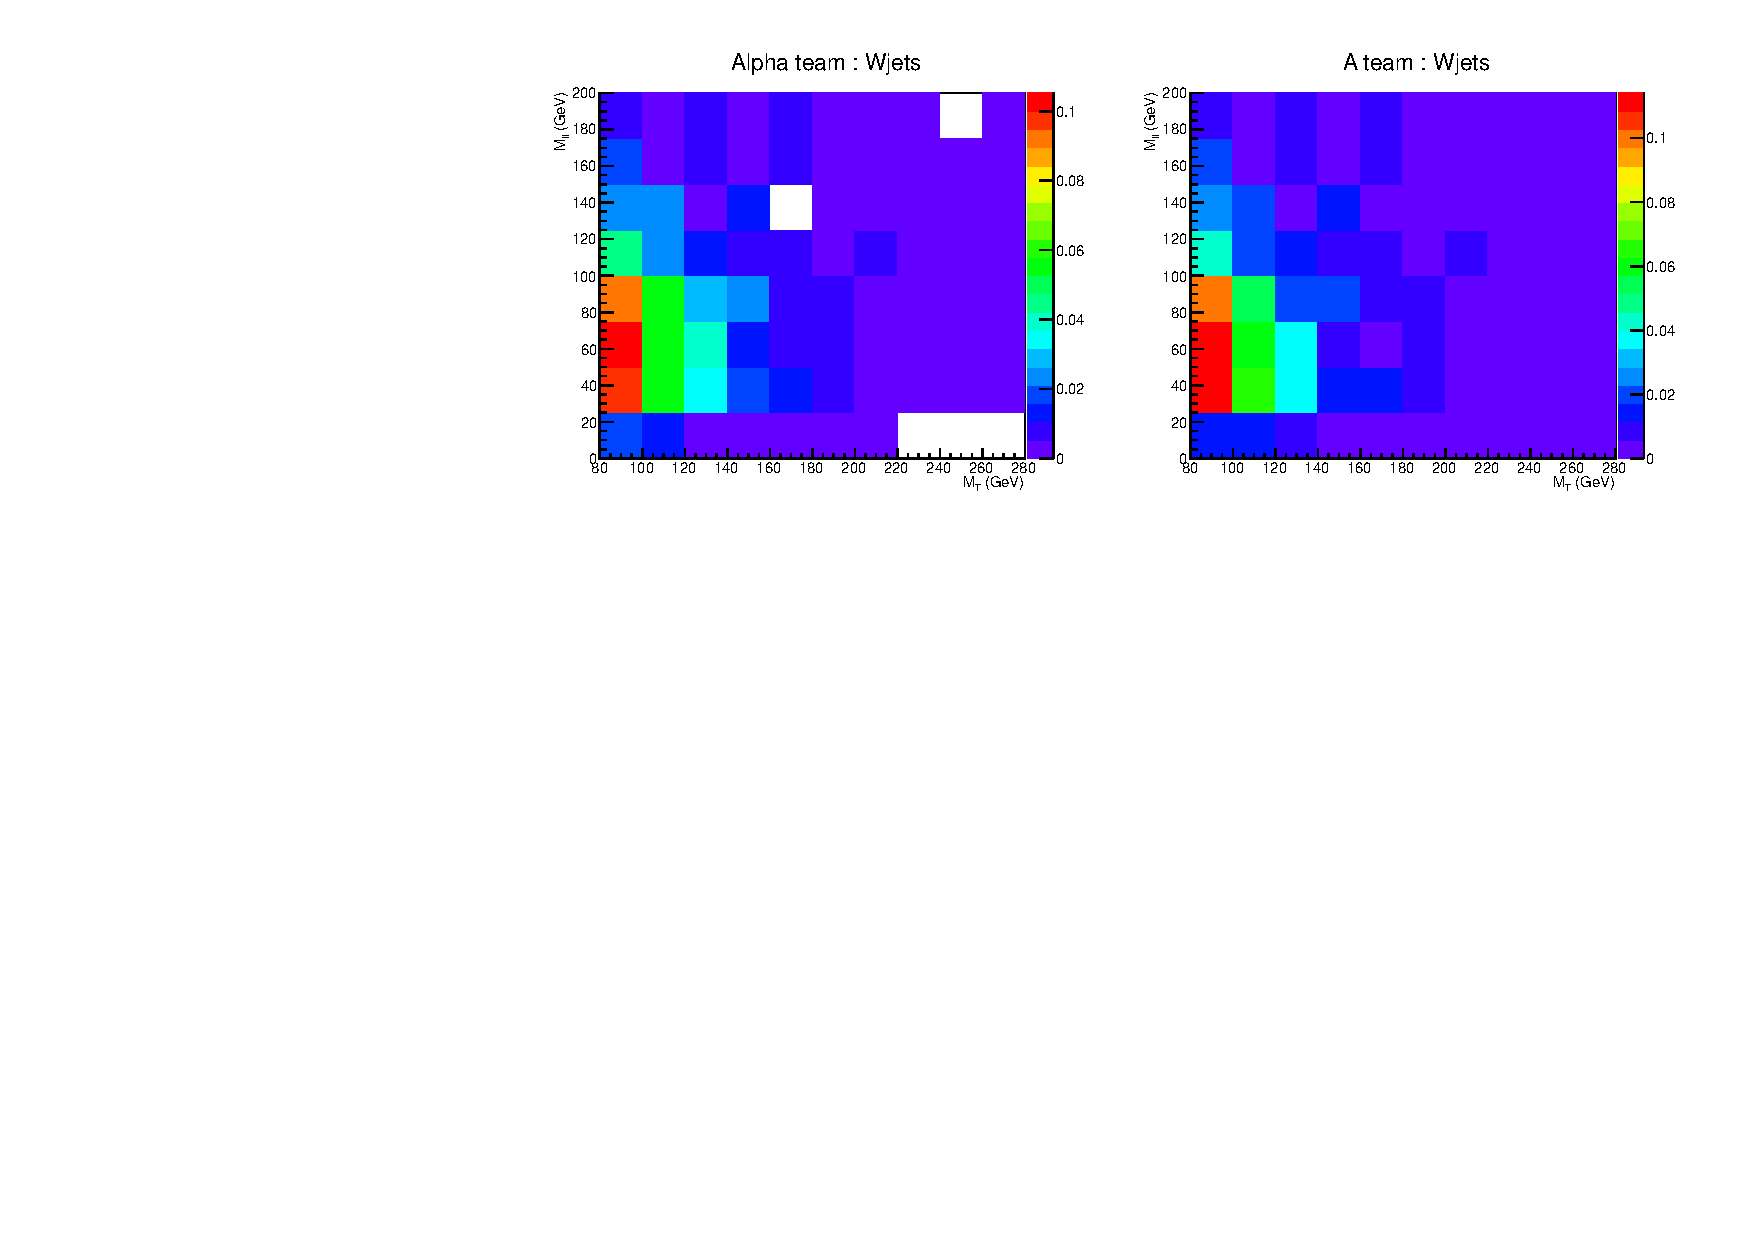
\includegraphics[width=.8\textwidth]{figures/compare_Wjets_1j.pdf}
} \\
\subfigure[Wgamma]{
\centering
\label{subfig:Wgamma_1j}
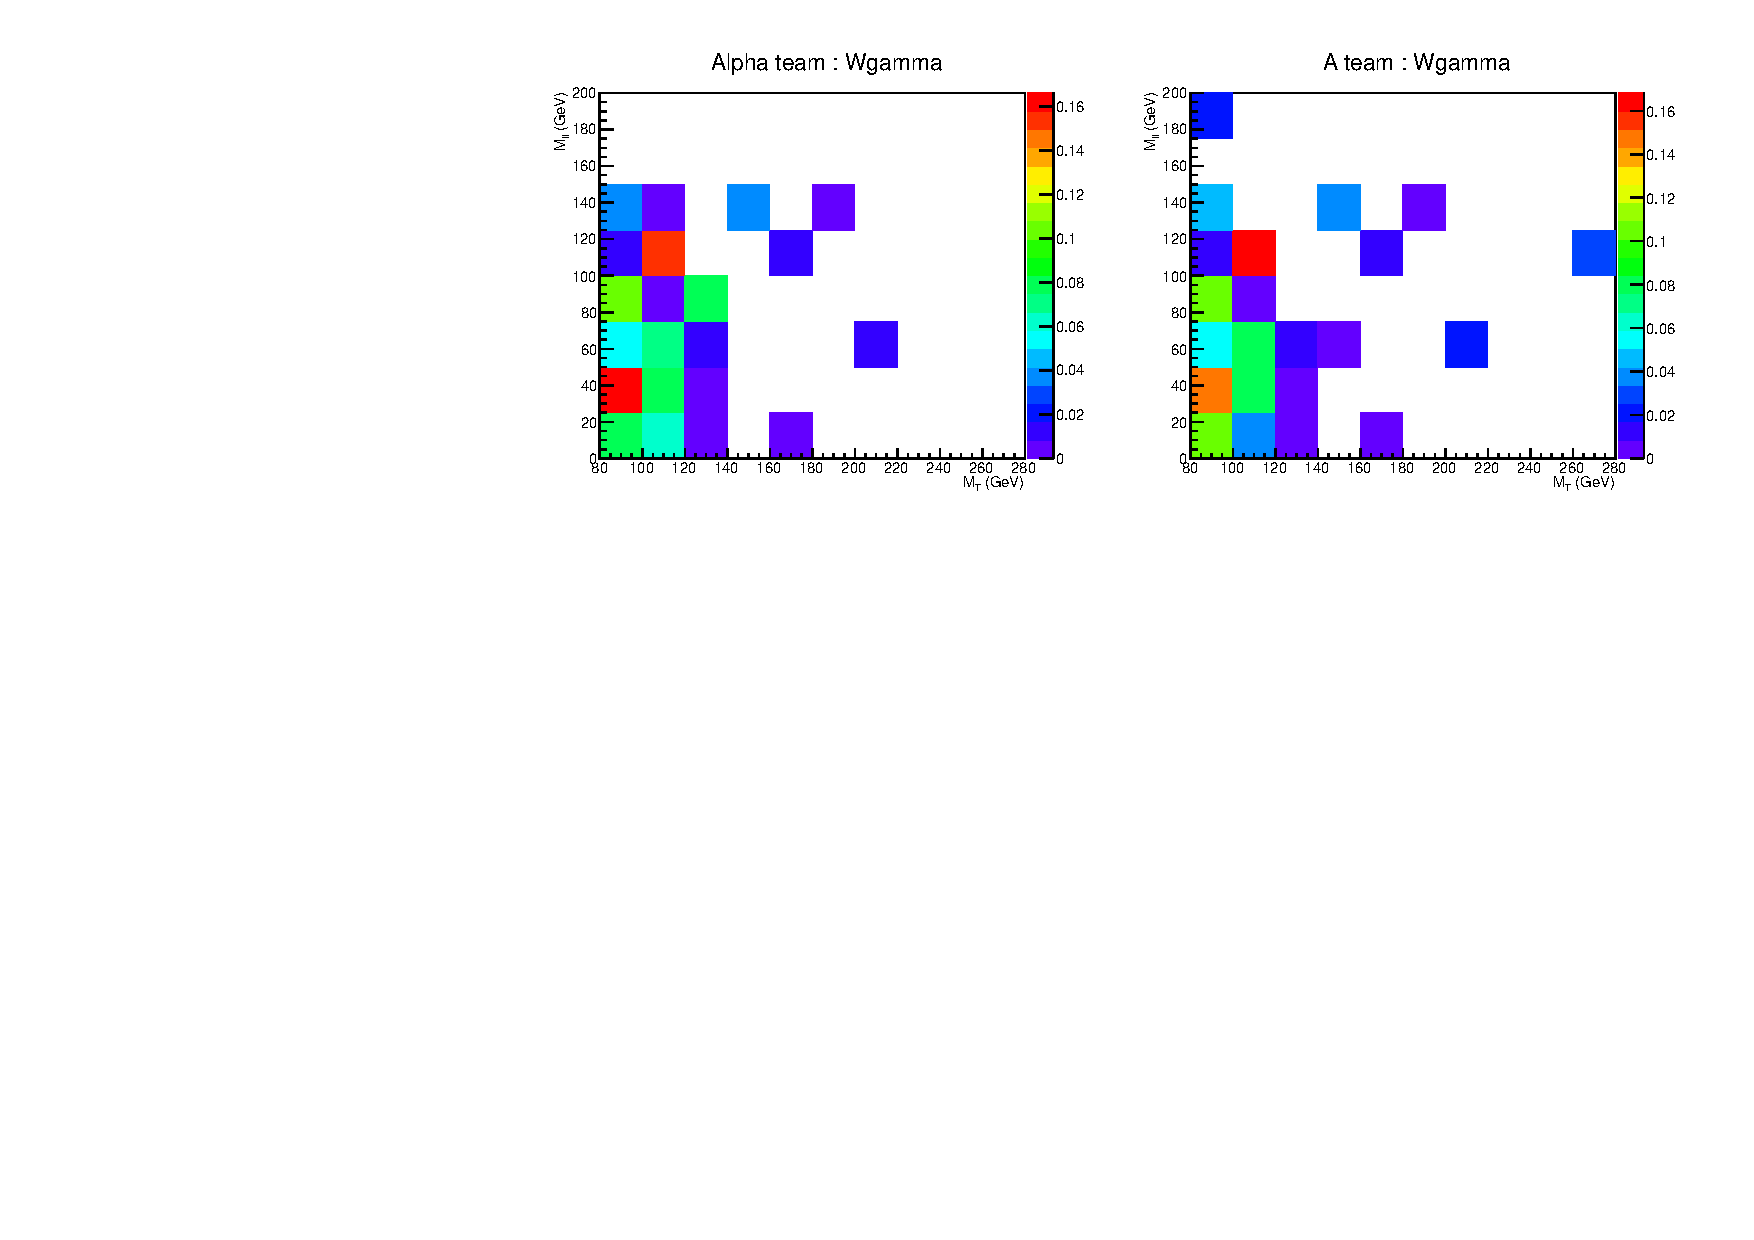
\includegraphics[width=.8\textwidth]{figures/compare_Wgamma_1j.pdf}
} \\

\caption{ The 2D ($m_{ll}, m_T$) templates for the Alpha team and A team in the 1-Jet bin with $m_H<300$ GeV. }
\label{fig:compare_temlates_1j}
\end{figure}
